 %%%%%%%%%%%%%%%%%%%%%%%%%%%%%%%%%%%%%%%%%
% Beamer Presentation
% LaTeX Template
% Version 1.0 (10/11/12)
%
% This template has been downloaded from:
% http://www.LaTeXTemplates.com
%
% License:
% CC BY-NC-SA 3.0 (http://creativecommons.org/licenses/by-nc-sa/3.0/)
%
%%%%%%%%%%%%%%%%%%%%%%%%%%%%%%%%%%%%%%%%%

%----------------------------------------------------------------------------------------
%	PACKAGES AND THEMES
%----------------------------------------------------------------------------------------

\documentclass{beamer}

\mode<presentation> {

% The Beamer class comes with a number of default slide themes
% which change the colors and layouts of slides. Below this is a list
% of all the themes, uncomment each in turn to see what they look like.

%\usetheme{default}
%\usetheme{AnnArbor}
%\usetheme{Antibes}
%\usetheme{Bergen}
%\usetheme{Berkeley}
%\usetheme{Berlin}
%\usetheme{Boadilla}
%\usetheme{CambridgeUS}
%\usetheme{Copenhagen}
%\usetheme{Darmstadt}
%\usetheme{Dresden}
%\usetheme{Frankfurt}
%\usetheme{Goettingen}
%\usetheme{Hannover}
%\usetheme{Ilmenau}
%\usetheme{JuanLesPins}
%\usetheme{Luebeck}
\usetheme{Madrid}
%\usetheme{Malmoe}
%\usetheme{Marburg}
%\usetheme{Montpellier}
%\usetheme{PaloAlto}
%\usetheme{Pittsburgh}
%\usetheme{Rochester}
%\usetheme{Singapore}
%\usetheme{Szeged}
%\usetheme{Warsaw}

% As well as themes, the Beamer class has a number of color themes
% for any slide theme. Uncomment each of these in turn to see how it
% changes the colors of your current slide theme.

%\usecolortheme{albatross}
%\usecolortheme{beaver}
%\usecolortheme{beetle}
%\usecolortheme{crane}
%\usecolortheme{dolphin}
%\usecolortheme{dove}
%\usecolortheme{fly}
%\usecolortheme{lily}
%\usecolortheme{orchid}
%\usecolortheme{rose}
%\usecolortheme{seagull}
%\usecolortheme{seahorse}
%\usecolortheme{whale}
%\usecolortheme{wolverine}

%\setbeamertemplate{footline} % To remove the footer line in all slides uncomment this line
%\setbeamertemplate{footline}[page number] % To replace the footer line in all slides with a simple slide count uncomment this line

%\setbeamertemplate{navigation symbols}{} % To remove the navigation symbols from the bottom of all slides uncomment this line
}

\usepackage{graphicx} % Allows including images
\usepackage{booktabs} % Allows the use of \toprule, \midrule and \bottomrule in tables
\usepackage{mathtools} 
\usepackage{subcaption}
\usepackage{multirow}

%----------------------------------------------------------------------------------------
%	TITLE PAGE
%----------------------------------------------------------------------------------------


\title[Intro to Neural Networks]{Intro to Neural Networks\\Machine Learning for Health Informatics}
\author{Anna Saranti}
\institute{Holzinger Group hci-kdd.org}
\date{01.04.2019}

\begin{document}

\begin{frame}
  \titlepage
  
  \begin{figure}[ht]
	\centering
    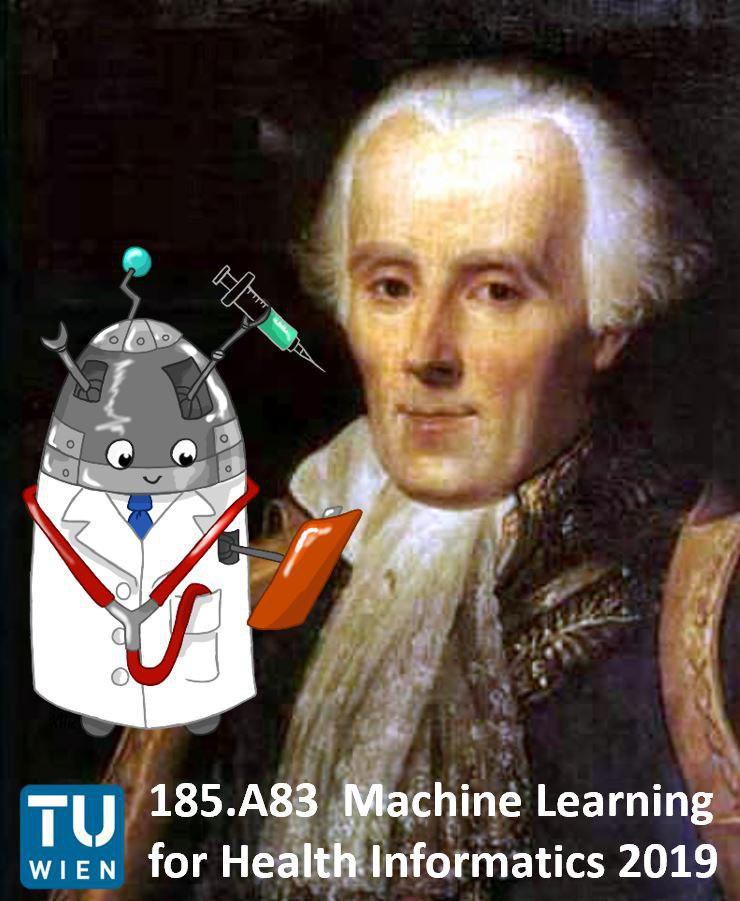
\includegraphics[width=2.5cm, height=3cm]{figures/HddKciLogo}
	\label{fig:HddKciLogo}
  \end{figure}
  
\end{frame}

%----------------------------------------------------------------------------------------
\section{Dataset splitting} 
%----------------------------------------------------------------------------------------
\begin{frame}
\frametitle{Dataset splitting and overfitting (1/5)}

\begin{figure}
  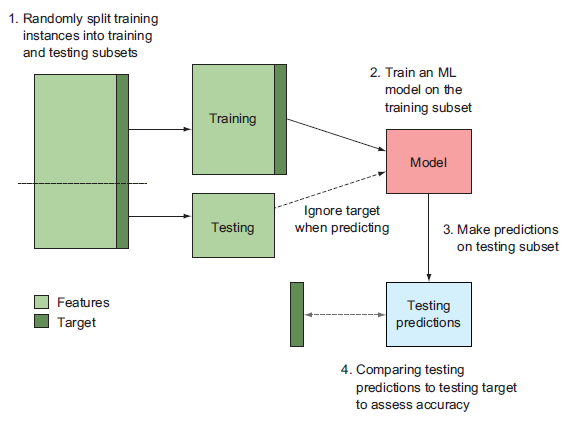
\includegraphics[width=6cm, height=4cm]{figures/ML_Workflow.png}
\end{figure}

\begin{figure}
  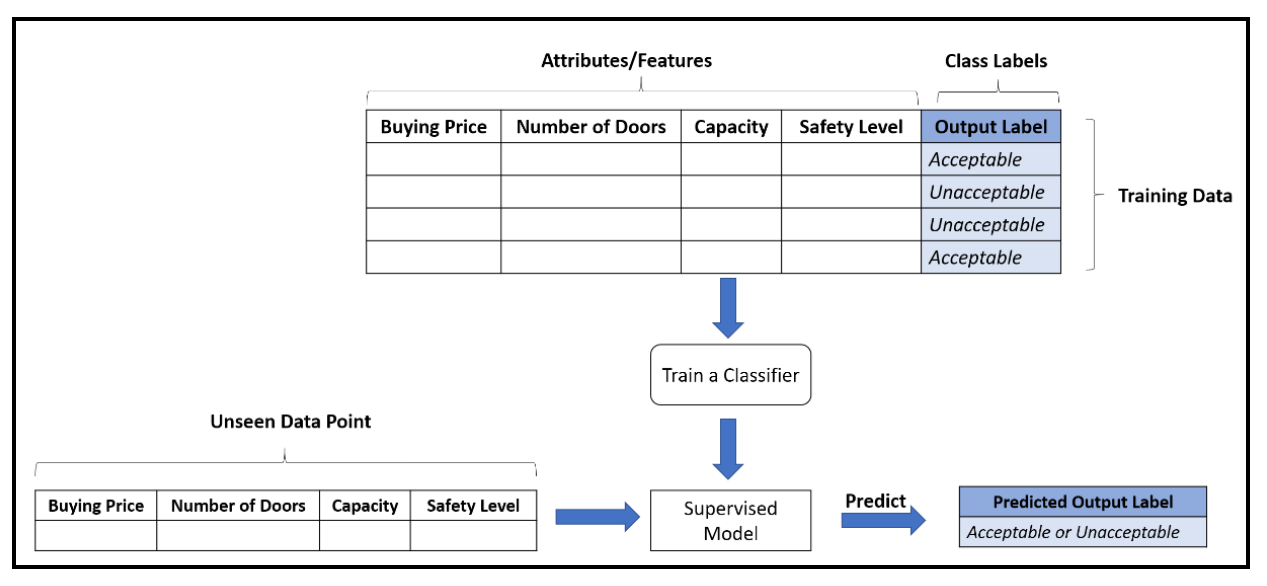
\includegraphics[width=6cm, height=3cm]{figures/DataSetsExample.png}
\end{figure}

\end{frame}

%----------------------------------------------------------------------------------------
\begin{frame}
\frametitle{Dataset splitting and overfitting (2/5)}

\begin{figure}
  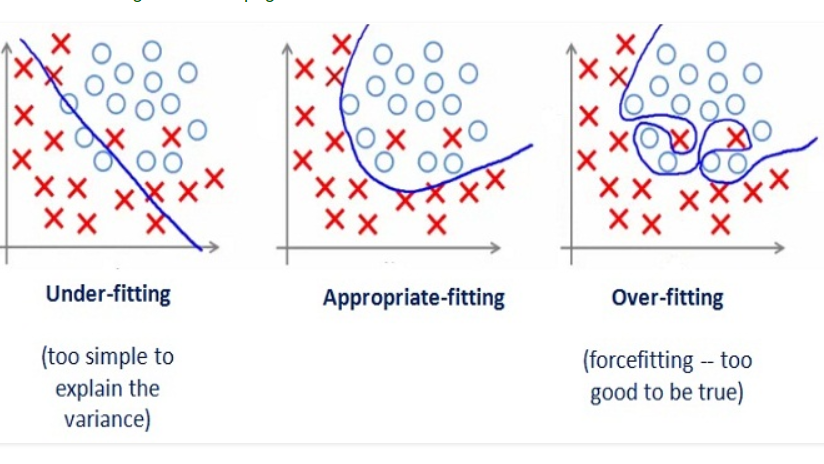
\includegraphics[width=8cm, height=4cm]{figures/OverFitting_1.png}
\end{figure}

\begin{figure}
  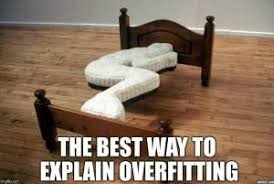
\includegraphics[width=4cm, height=3cm]{figures/OverFitting_2.jpg}
\end{figure}

\end{frame}

%----------------------------------------------------------------------------------------
\begin{frame}
\frametitle{Dataset splitting and overfitting (3/5)}

\begin{itemize}
\item Pretend that part of the data is not seen yet
\item The model makes a statement about this set - does this hold?
\end{itemize}

\begin{figure}
  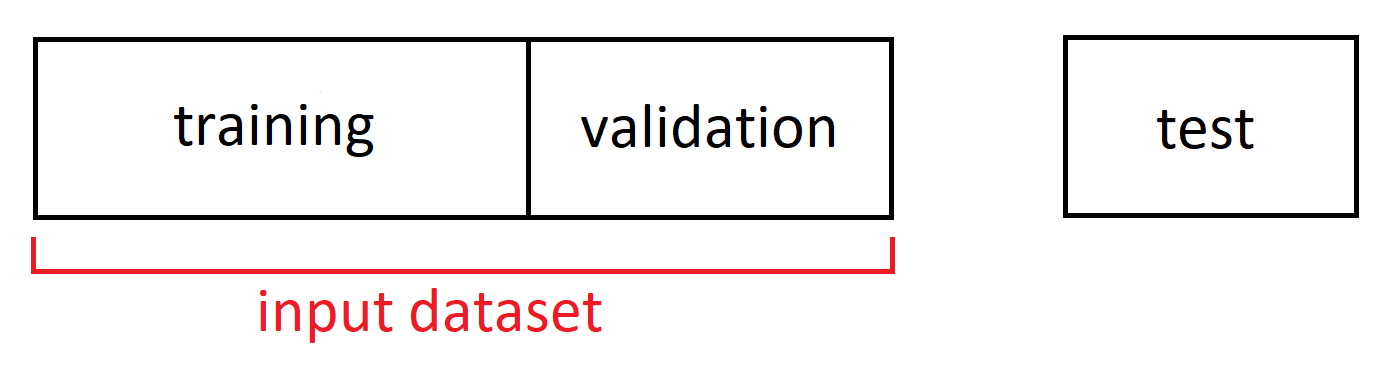
\includegraphics[width=6cm, height=1.5cm]{figures/TrainingValidationTestSet.png}
\end{figure}

\begin{figure}
  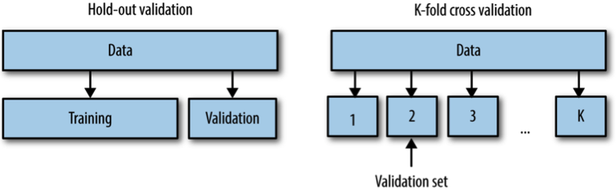
\includegraphics[width=9cm, height=3cm]{figures/K-Fold_CrossValidation.png}
\end{figure}

\end{frame}

%----------------------------------------------------------------------------------------
\begin{frame}
\frametitle{Dataset splitting and overfitting (4/5)}

\begin{itemize}
\item \url{https://scikit-learn.org/stable/}
\item \texttt{sklearn.model\_selection.train\_test\_split}
\item \texttt{sklearn.model\_selection.StratifiedShuffleSplit}, \texttt{sklearn.model\_selection.StratifiedKFold}
\item Training and test set should have roughly the same percentage of data in each class
\item Beware that shuffling may spread a characteristic that exists in one part of the data in all the folds!
\end{itemize}
\end{frame}

%----------------------------------------------------------------------------------------
\begin{frame}
\frametitle{Dataset splitting and overfitting (5/5)}

\begin{itemize}
\item Overfitting: Model memorizes and does not generalize to unseen data (test set)
\end{itemize}

\begin{figure}
  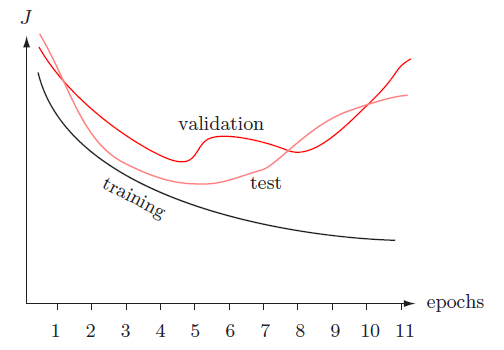
\includegraphics[width=4.2cm, height=3cm]{figures/NNError.png}
\end{figure}

\end{frame}
%----------------------------------------------------------------------------------------

%----------------------------------------------------------------------------------------
\section{Supervised ML - Classification} 
%----------------------------------------------------------------------------------------
\begin{frame}
\frametitle{Classification Metrics}

\begin{itemize}
\item \textbf{Don't use accuracy!} The ratio of correct predictions) is not enough when the dataset is imbalanced. 
If a data set contains 90\% of samples belonging to a single class, the classifier that by default (no programmed logic) only chooses this class, has 90\% accuracy.
The classifier is not informative - did not learn anything.
\item Confusion matrix - compare the predicted class with the actual class:

\begin{table}[H]
\begin{center}
\begin{tabular}{|c|c|c|c|}
\cline{3-4}
\multicolumn{2}{c|}{} & \multicolumn{2}{c|}{ \textbf{Predicted} } \\
\cline{3-4}
\multicolumn{2}{c|}{} & Negative & Positive \\
\hline
\multirow{2}{*}{\textbf{Actual}} & Negative & TN & FP \\
\cline{2-4}
& Positive & FN & TP \\
\hline
\end{tabular}
\end{center}
\end{table}

\item Mutual information - measures how many bits the classifier's output conveys about the predicted target.\\
Helps comparing multi-class classifiers, not directly possible with confusion matrices $2 \times 2$, $4 \times 4$.
\end{itemize}

\end{frame}
%----------------------------------------------------------------------------------------
\begin{frame}
\frametitle{Neural Network for Classification (1/5)}

One artificial neuron
\begin{figure}
  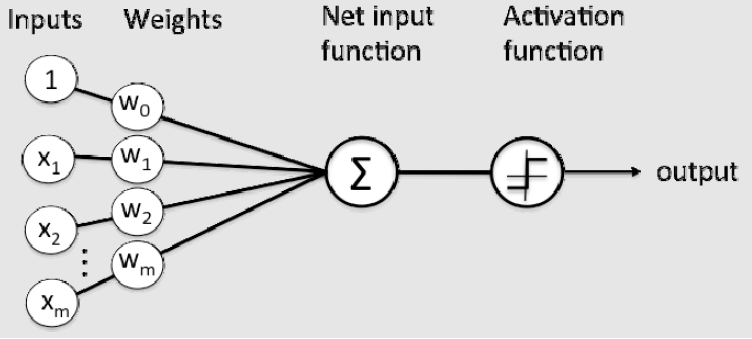
\includegraphics[width=8cm, height=4cm]{figures/OneNeuron.png}
\end{figure}

\begin{itemize}
\item Prediction: $\hat{y} = \textrm{activation}(\sum_i x_i w_i + b) = f(x)$
\item Error: $J = y - \hat{y} $
\end{itemize}

\end{frame}
%----------------------------------------------------------------------------------------
\begin{frame}
\frametitle{Neural Network for Classification (2/5)}

\begin{itemize}
\item Learn a non-linear function of the input that approximates the output/target variable
\item Architecture is not known, it must be learned as the parameters
\item The input must be numeric and has to be scaled
\end{itemize}

\begin{figure}
  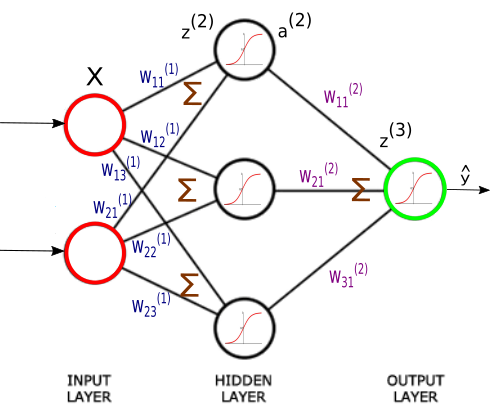
\includegraphics[width=4cm, height=3cm]{figures/NNArch.png}
\end{figure}

\end{frame}
%----------------------------------------------------------------------------------------
\begin{frame}
\frametitle{Neural Network for Classification (3/5)}

\begin{itemize}
\item Various non-linear activation functions (sigmoid, tanh, ReLU)
\item Different methods to adapt step-wise the parameters to minimize the error - 
Bigger steps in the beginning, smaller in the end.
\item Different architectures depending on the problem (CNN, RNN)
\item Adjust a little the parameters/weights a little according to the error (difference) of the computed with the actual (target)
(Back-propagation)
\end{itemize}

\begin{figure}
  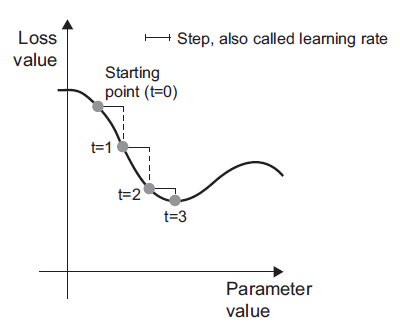
\includegraphics[width=5cm, height=4cm]{figures/GradientDescent.png}
\end{figure}

\end{frame}
%----------------------------------------------------------------------------------------
\begin{frame}
\frametitle{Neural Network for Classification (4/5)}

\begin{figure}
  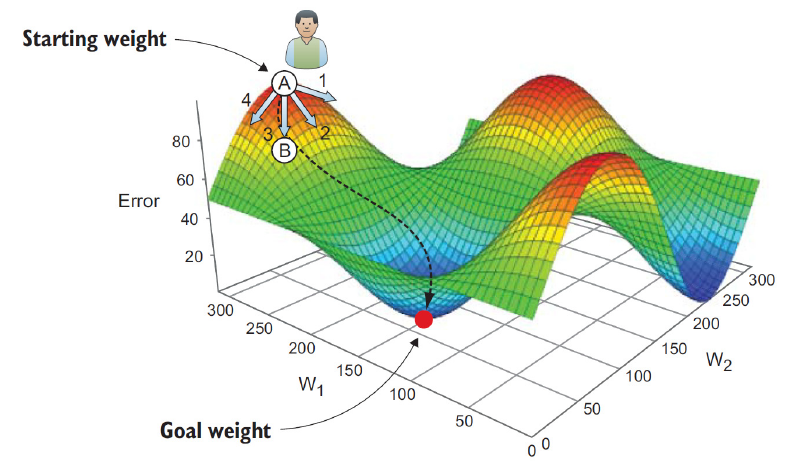
\includegraphics[width=5cm, height=3cm]{figures/GD_1.png}
\end{figure}

\begin{figure}
  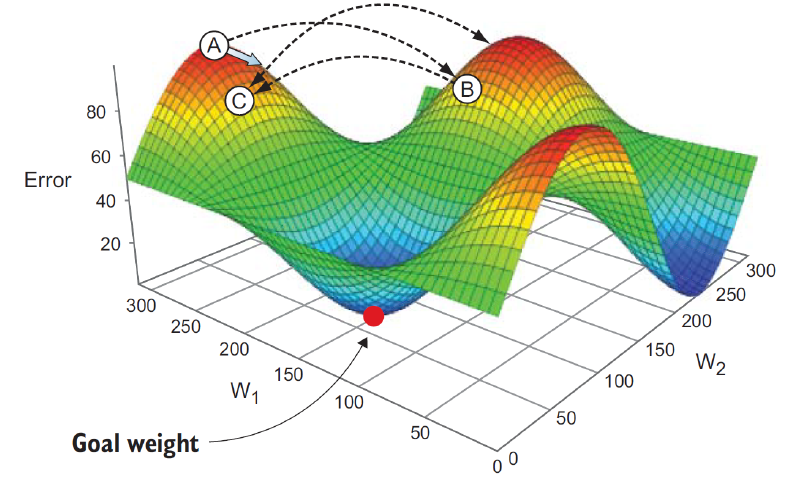
\includegraphics[width=5cm, height=3cm]{figures/GD_2.png}
\end{figure}

\end{frame}
%----------------------------------------------------------------------------------------
\begin{frame}
\frametitle{Neural Network for Classification (5/5)}

\begin{itemize}
\item Repeat until the parameters do not change a lot
\item Don't learn too much - don't overfit.
\item Check the output of the hidden layers and the values of the weights to discover some patterns 
\end{itemize}

\end{frame}

%----------------------------------------------------------------------------------------
\begin{thebibliography}{99} % Beamer does not support BibTeX so references must be inserted manually as below

\begin{frame}
\frametitle{References}

\bibitem[Duda, Richard O., Peter E. Hart, and David G. Stork]{p1} Duda, Richard O., Peter E. Hart, and David G. Stork (2012)
\newblock Pattern classification [Chapter 6]
\newblock \emph{John Wiley \& Sons}

\bibitem[Christopher M. Bishop, 2006]{p2} Christopher M. Bishop (2006)
\newblock Pattern Recognition and Machine Learning [Chapter 5]
\newblock \emph{Springer}

\bibitem[Aur\'elien G\'eron, 2017]{p3} Aur\'elien G\'eron (2017)
\newblock Hands-On Machine Learning with Scikit-Learn and TensorFlow
\newblock \emph{O'Reilly}

\bibitem[David J.C. MacKay]{p4} David J.C. MacKay (2003)
\newblock Information Theory, Inference, and Learning Algorithms
\newblock \emph{Cambridge University Press}

\end{frame}

\end{thebibliography}

%----------------------------------------------------------------------------------------

\end{document} 